\chapter{Experimental Evaluation}
\label{ch:experimental-evaluation}

Chapters~4 and~5 described kernel collection and user-space processing
separately. This chapter evaluates them together in a controlled container
environment. A reproducible node-local scenario is followed from workload
execution to monitored evidence, collective alert and measured container
resources.

\section{Evaluation Objectives and Experimental Protocol}
\label{sec:evaluation-objectives-protocol}

The evaluation addresses three questions:
\begin{itemize}
    \item Can the monitoring agent observe security-relevant activity generated inside 
    another container when the Pod does not share its process namespace with the host?
    \item Can the configured collective detector assemble the expected sequence of process and
    file events while leaving a controlled benign interaction without an alert?
    \item How does exact kernel-side \gls{uid} filtering affect the resources
    charged to the monitor container during the attack workload?
\end{itemize}

The three questions use different evidence boundaries. Cross-container
visibility is established from decoded records carrying both container and host
process identities. Detector behaviour is assessed from the ordered evidence
inside each alert and from the absence of alerts in the selected benign
windows. Resource use is measured independently through cgroup and node
counters. Keeping these observations separate avoids treating successful
collection, a detector match and application-level exploit output as the same
experimental outcome.

The functional campaign used three benign and four exploit windows. Each had a
distinct run identifier and retained trigger output, standard error and
time-bounded container logs. The performance campaign used five rounds of
three profiles: filtered monitor, unfiltered monitor and no monitor. The
starting profile shifted between rounds, producing fifteen cyclically ordered
runs. The Pod was recreated and allowed to become ready before each run.

After a ten-second warm-up, the protocol selected samples whose endpoint fell
inside the externally recorded workload interval. Sampling was nominally once
per second, with some variation from reads through Minikube \gls{ssh}. The local
acceptance gate was 5\% of one core for mean \gls{cpu} time charged to the monitor
cgroup; it does not represent total host overhead. Results use the five run
means per profile, with sample standard deviation describing only variation
among those runs.

Experimental inputs were the trigger scenario and selected monitor profile.
The functional campaign recorded event evidence and alert counts; the
performance campaign recorded cgroup CPU, memory, \gls{rss}, PID count, node CPU
and workload duration. Host, cluster allocation, images, policy, detector and
synthetic flag were held fixed. Run identifiers and \gls{utc} boundaries linked
scenario output to the relevant log window, excluding older alerts from later
runs.

\section{Experimental Testbed}
\label{sec:evaluation-testbed}

The experiment used the development target as the host of a single-node
Minikube cluster created through the Docker driver
\cite{minikube_docker_driver}. Table~\ref{tab:evaluation-environment} records
the exact software versions and allocated resources. No result depends on
functionality introduced after the development baseline.

The \texttt{aes-beta-lab} Pod contained a vulnerable target, an input trigger
and the monitor. The trigger contacted the target over Pod-local loopback on
port 1337. The target and trigger shared the Pod network but not a process
namespace, and the Pod did not join the host network or process namespace
\cite{kubernetes_pod_networking,kubernetes_process_namespace}.

\begin{figure}[H]
    \centering
    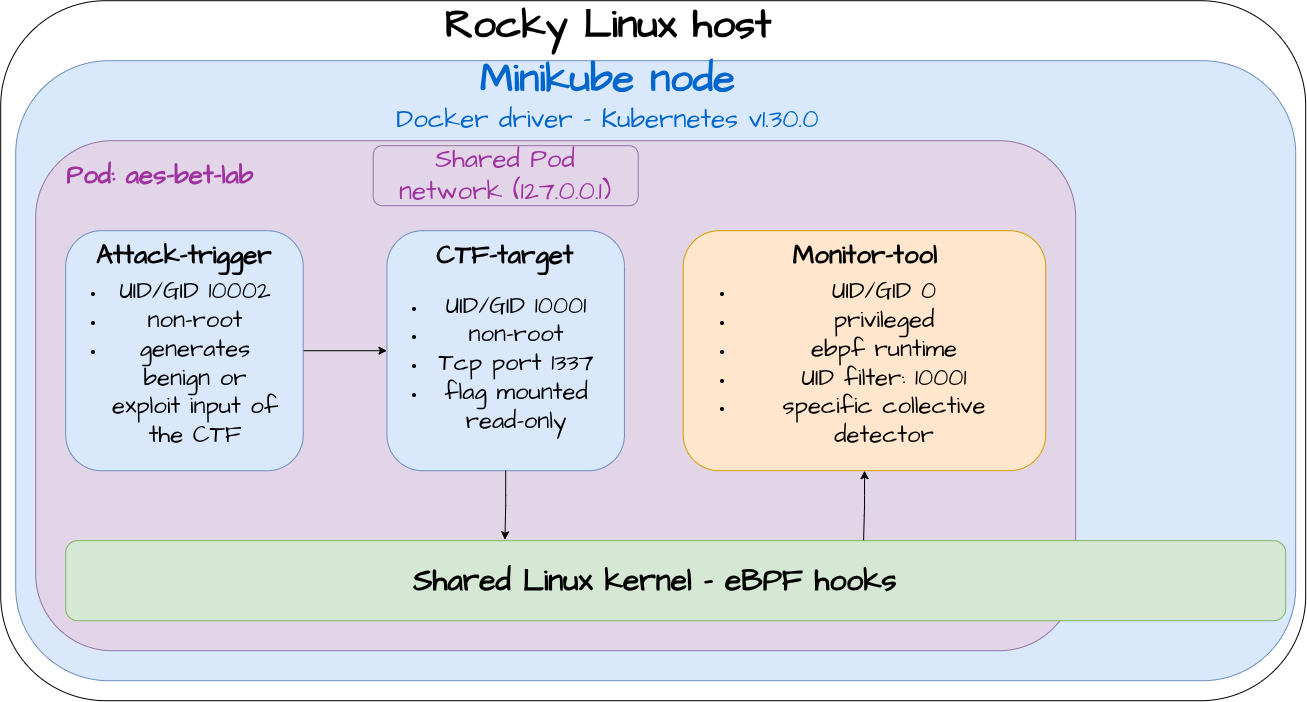
\includegraphics[
        width=0.95\textwidth,
        keepaspectratio
    ]{figures/chapter6/kubernetes-testbed-topology.drawio.png}
    \caption[Minikube experimental testbed]
    {Experimental topology of the three-container Pod and its relationship
    with the shared node kernel.}
    \label{fig:evaluation-kubernetes-testbed}
\end{figure}

The target and trigger were deliberately constrained as non-root containers,
whereas the monitor required privileged access to host kernel interfaces. The
exact identities, security contexts and mounts appear in
Table~\ref{tab:evaluation-environment}. This laboratory configuration does not
represent a least-privilege deployment \cite{kubernetes_privileged_containers}.
The default service-account token also remained mounted, although no evaluated
scenario depended on Kubernetes \gls{api} access.

\begin{table}[H]
    \centering
    \small
    \renewcommand{\arraystretch}{1.15}
    \begin{tabularx}{\textwidth}{@{}p{0.22\textwidth}X@{}}
        \toprule
        \textbf{Dimension} & \textbf{Experimental configuration} \\
        \midrule
        Host & Rocky Linux 8.10; kernel recorded as
        \path{4.18.0-553.137.1.el8_10.x86_64} \\
        Cluster & Minikube v1.38.1; Docker driver; Kubernetes v1.30.0;
        one node with two requested CPUs and 4096~MiB \\
        Pod isolation & Three containers; \texttt{hostPID: false};
        \texttt{hostNetwork: false}; \texttt{shareProcessNamespace: false} \\
        Target and trigger & Non-root UIDs 10001 and 10002; read-only root
        filesystems; no privilege escalation; all capabilities dropped \\
        Monitor & Privileged UID 0; unconfined seccomp; host BTF, bpffs and
        tracefs mounted into the container \\
        Monitored event set & \texttt{sched\_process\_exec},
        \texttt{security\_file\_open} and \texttt{open} \\
        Workload provenance & AES-beta from openECSC-2024; recorded revision
        \texttt{2602f22c}; checked binary,
        loader and C library; synthetic flag \\
        \bottomrule
    \end{tabularx}
    \caption{Experimental environment and controlled configuration.}
    \label{tab:evaluation-environment}
\end{table}

Before image construction, the public challenge revision was recorded and the
binary, dynamic loader and C library were checked against fixed hashes. The
preparation script verifies these artefacts, though not the Git revision of the
source checkout. The applied Pod, policy and detector were preserved with
configuration hashes, and the running Pod record retained all three image
identities. The flag was synthetic rather than a competition secret. Full
hashes, manifests, commands and image identifiers remain in the reproducibility
material.

The Pod declared resource requests but no limits. Measurements therefore
describe use under contention on the allocated node, not enforcement at a fixed
container ceiling. No snapshot of realised Kubernetes allocatable capacity was
archived.

\section{Controlled AES-beta Scenario}
\label{sec:evaluation-workload}

AES-beta is a public Capture the Flag challenge adapted as a controlled
process-monitoring workload \cite{openecsc2024_aes_beta}. Benign runs exercised
the service without reading the mounted flag. Exploit runs drove the target to
invoke a shell, execute \texttt{cat} and access
\path{/opt/aes-beta/flag}. Payload construction was fixed; the experiment
examined the resulting host behaviour.

The policy admitted three logical events. The detector required four ordered
observations from UID 10001 within five seconds: successful transitions to
\path{/bin/sh} and \path{/bin/cat}, a \texttt{security\_file\_open} observation
for the resolved flag path, and an \texttt{open} event for caller pathname
\texttt{flag} with a non-negative return. The security hook showed mediation;
the returned file descriptor supplied success evidence at the syscall
boundary.

The sequence used \texttt{process\_tree} correlation. All four records in each
alert shared one host \gls{pid}, so this experiment exercised its same-process
branch, not parent-to-child correlation. Alerts carried high severity and
ATT\&CK identifiers TA0002, TA0009, T1059.004 and T1005. These classify the
sequence in the \gls{attack} vocabulary \cite{strom2020attack}; they do not
measure detector coverage.

Unlike direct invocation of the monitored commands, this scenario required the
evidence to originate from the vulnerable service rather than the trigger.
Challenge artefacts and runtime dependencies were fixed, and success used a
synthetic value with no operational consequence.

\section{Functional Evaluation}
\label{sec:evaluation-functional}

\subsection{Cross-Container Event Visibility}
\label{subsec:evaluation-cross-container-visibility}

The visibility test captured 7,289 records, of which nine had process UID
10001. They described a directly invoked \texttt{cat} in the target container,
including executable transition, resolved flag object and successful open. The
process had container PID 327 and host PID 3016236, preserving both its
namespace-relative and node-local identities.

This confirms visibility into the target container with \texttt{hostPID: false}
and no shared Pod process namespace. All containers still ran on one Minikube
node and shared its kernel; cross-node visibility was not tested.

\subsection{Collective Detector Validation}
\label{subsec:evaluation-collective-detector}

Inspection of the exploit alerts showed the intended four-stage evidence. In
the first run, executable transitions identified \path{/bin/sh} and
\path{/bin/cat}, the mediation event identified the resolved flag object, and
the final \texttt{open} returned file descriptor 2. That return supplied the
success evidence absent from the LSM entry observation.

The first-to-last event spans were 0.941, 0.625, 0.650 and 0.725~ms, all inside
the five-second window. These are differences between kernel timestamps, not
detector or delivery latency. Every alert retained one host PID across its
evidence, confirming same-process correlation in this scenario.

The monitor and exploit client observed different stages. The alert establishes
the shell and \texttt{cat} transitions and a successful open, not delivery of
file contents to the trigger. In E3 the sequence completed, but the client
received an empty flag value and exited with status 1.

\subsection{Benign Control and Repeated Runs}
\label{subsec:evaluation-functional-repetitions}

Table~\ref{tab:evaluation-functional-runs} reports the seven functional
windows, including client outcome, alert count and recorded perf-loss
diagnostics.

\begin{table}[H]
    \centering
    \footnotesize
    \setlength{\tabcolsep}{4pt}
    \renewcommand{\arraystretch}{1.14}
    \begin{tabularx}{\textwidth}{@{}p{0.09\textwidth}Xr r r r@{}}
        \toprule
        \textbf{Run} & \textbf{Scenario outcome} &
        \textbf{Internal (ms)} & \textbf{Wall (ms)} &
        \textbf{Alerts} & \textbf{Loss diag.} \\
        \midrule
        B1 & Benign pass & 17 & 1,118 & 0 & 0 \\
        B2 & Benign pass & 11 & 1,024 & 0 & 0 \\
        B3 & Benign pass & 11 & 1,038 & 0 & 0 \\
        E1 & Exploit pass; flag returned & 48,543 & 49,627 & 1 & 0 \\
        E2 & Exploit pass; flag returned & 51,584 & 52,759 & 1 & 0 \\
        E3 & Empty client output; status 1 & 49,509 & 50,591 & 1 & 0 \\
        E4 & Diagnostic exploit pass; flag returned & 49,548 & 50,754 & 1 & 0 \\
        \bottomrule
    \end{tabularx}
    \caption{Results of the repeated functional windows. Every exploit alert
    contained four ordered evidence events.}
    \label{tab:evaluation-functional-runs}
\end{table}

Within these runs, the pipeline completed the collective sequence only in the
exploit windows. This is not a detection-accuracy estimate: the detector
targeted a known scenario, the benign control was narrow and no independent
holdout set was used.

\section{Performance Evaluation}
\label{sec:evaluation-performance}

\subsection{Metrics, Sampling and Benchmark Profiles}
\label{subsec:evaluation-performance-method}

The filtered profile enabled the exact UID 10001 kernel filter. The unfiltered
profile kept the same policy, detector, alert mode and workload without that
filter. The no-monitor profile removed the monitor container and provided only
workload context. Before each run, the Pod was recreated under the selected
profile and allowed to reach readiness. Profile order rotated over five rounds
rather than being randomised.

Filtered and unfiltered runs differed by the intended kernel-side UID setting.
Removing the monitor also removed its host mounts, so the no-monitor profile was
not an otherwise identical overhead control. It was retained to show target
workload scale and variability.

The primary performance comparison is therefore between the two monitored
profiles. Both execute the same target workload and user-space detector path;
the intended difference is whether unrelated UIDs are rejected in the common
kernel initialisation path. This comparison measures work charged to the
monitor container after that change. The no-monitor profile cannot answer the
same question, but it helps show whether the target workload and node were
stable enough to interpret the monitored runs.

Container CPU divided cgroup-v1 \texttt{cpuacct.usage} deltas by wall-clock
deltas \cite{linux_cgroup_v1_cpuacct}; 100\% represents one fully used core.
Node CPU came from \path{/proc/stat}, with the complete two-core node mapped to
0--100\%. Cgroup memory and resident set size (\gls{rss}) were recorded
separately because charged pages may extend beyond the resident process set.
PID count and internal workload duration were also retained.

In monitored runs, the primary cgroup belonged to the monitor and the target
was sampled separately. Without the monitor, the primary cgroup belonged to the
target. Its CPU and memory cannot be subtracted from the monitor columns as an
overhead baseline.

\subsection{Resource Consumption and Workload Duration}
\label{subsec:evaluation-resource-results}

Table~\ref{tab:evaluation-performance-results} summarises the replicas. Each CPU
mean and standard deviation uses five per-run means.

\begin{table}[H]
    \centering
    \scriptsize
    \setlength{\tabcolsep}{3.5pt}
    \renewcommand{\arraystretch}{1.15}
    \begin{tabularx}{\textwidth}{@{}p{0.19\textwidth}p{0.18\textwidth}p{0.18\textwidth}p{0.20\textwidth}X@{}}
        \toprule
        \textbf{Profile and metric owner} &
        \textbf{CPU mean $\pm$ \gls{sd}} &
        \textbf{Median; range} &
        \textbf{Campaign max memory / \gls{rss}} &
        \textbf{Workload duration mean $\pm$ \gls{sd}} \\
        \midrule
        Filtered monitor & 0.39\% $\pm$ 0.02 &
        0.39\%; 0.36--0.41\% & 100.51 / 39.36~MiB &
        54.85 $\pm$ 4.09~s \\
        Unfiltered monitor & 4.87\% $\pm$ 0.11 &
        4.89\%; 4.73--4.98\% & 112.16 / 46.02~MiB &
        61.33 $\pm$ 3.04~s \\
        No-monitor target & 34.80\% $\pm$ 3.57 &
        35.90\%; 28.66--37.74\% & 19.02 / 6.88~MiB &
        56.27 $\pm$ 7.22~s \\
        \bottomrule
    \end{tabularx}
    \caption{Replicated performance results, with five runs per profile. CPU
    and duration values summarise per-run observations; memory and \gls{rss} are the
    maxima across all selected samples and replicas. Metrics belong to the
    container named in the first column.}
    \label{tab:evaluation-performance-results}
\end{table}

The memory and \gls{rss} entries are campaign maxima, not steady-state
requirements. Values in the no-monitor row belong to the target and are
included only as workload context.

Mean node CPU was near saturation in every profile: 94.70\% filtered, 95.11\%
unfiltered and 94.89\% without the monitor. Workload duration varied between
replicas. The small sample, variable workload cost and high utilisation prevent
interpreting the shorter filtered mean as a monitor effect.

\subsection{Observed Difference with Kernel-Side UID Filtering}
\label{subsec:evaluation-uid-filter}

All five filtered run means fell below the project-defined 5\% gate. Under the
scripted profiles, exact UID admission was associated with approximately 92.0\%
lower mean monitor-cgroup CPU than the unfiltered profile. Both profiles
appeared in every round, but the archive lacks the rendered monitor
configuration and image identity for each replica. The comparison shows a
strong association under the intended profiles, not proof that the filter alone
caused the difference.

Kernel execution is not fully represented by the monitor cgroup, and host-level
kernel cost was not isolated. The 5\% result applies only to measured
monitor-cgroup CPU in the filtered profile.

Each of the ten monitored performance runs still produced one alert, with no
matching textual perf-loss diagnostic. Thus, the configured evidence remained
available in these runs; transport loss was not independently measured.

\section{Discussion of Results}
\label{sec:evaluation-discussion}

Host-level observation did not depend on exposing the host process namespace to
the target Pod. The retained host identity supported local correlation without
treating a container PID as globally meaningful. Separating executable
transition, security mediation and syscall outcome also prevented the LSM
observation alone from being interpreted as completed file access.

Early UID admission was associated with substantially less work charged to the
monitor cgroup, consistent with rejecting unrelated events before transport and
user-space processing. Incomplete per-run configuration provenance and
near-saturated node utilisation prevent a stronger causal or total-overhead
claim.

E3 illustrates the evidence boundary directly. Its alert represented the
observed host operations, including a successful file descriptor return; the
empty client result arose later, outside the detector sequence. Kernel evidence
and end-to-end application success must therefore be reported separately.

\section{Threats to Validity and Current Limitations}
\label{sec:evaluation-threats-validity}

\noindent\textbf{Internal validity.}
Profiles rotated cyclically rather than randomly. Pod recreation reduced
container-state carry-over but not host load, cache effects or exploit
variation. Minikube \gls{ssh} sampling sometimes exceeded the nominal one-second
period. Selection used each sample's endpoint although its CPU value covered
the preceding interval, so the first sample may include pre-workload activity
and the final partial interval may be absent. The node was near saturation in
all profiles. E3 also showed that client output can fail after the monitored
host sequence completes.

\medskip
\noindent\textbf{Construct validity.}
Monitor-cgroup CPU is not total monitoring overhead, and no-monitor target
metrics are not a monitor baseline. Cgroup memory and \gls{rss} cover different
boundaries; event timestamp spans are not detector or output latency; absence
of a loss diagnostic is not proof of loss-free transport. Functional results
also depend on distinguishing LSM mediation from the returned syscall result.

\medskip
\noindent\textbf{External validity.}
The experiment covered one Rocky Linux build, one Docker-backed Minikube node,
one Kubernetes version, one public \gls{ctf} challenge and a detector tailored
to it. The benign control was narrow. Alternative kernels, long-running or
production workloads and multi-node deployments were not evaluated, so the
results apply to this node-local scenario.

\medskip
\noindent\textbf{Conclusion validity.}
Five replicas per performance profile and seven functional windows support
descriptive comparison, not inferential statistics or accuracy rates. The
observed difference is specific to the selected events, UID, workload and node.
Missing per-run rendered configuration and image identity prevent independent
confirmation that filtering was the only realised difference. Target CPU,
memory and duration differences are not causal performance evidence. ATT\&CK
metadata classifies alerts but does not validate coverage.

\section{Evaluation Summary}
\label{sec:evaluation-summary}

The experiment established node-local visibility into the target container and
showed that the configured sequence distinguished the controlled exploit from
the selected benign interaction. The filtered profile remained below the local
CPU gate and was associated with markedly lower monitor-cgroup CPU than the
unfiltered profile. Total overhead, broad detection accuracy and multi-node
behaviour were not established. Chapter~7 draws conclusions from these bounded
results and identifies future work.
